% Preamble needs:
% \usepackage{tikz}
% \usetikzlibrary{positioning,calc,arrows.meta}

\begin{figure}
\begin{tikzpicture}
	

\begin{scope}[shift={(3,0)}]
	% Draw the inner circle (radius = 1.5)
	\shade[Rubric_circlegradient_Challenge_Pertubation] circle (1.5);
	
	% Center node text   
	\node at (0,0) [
	font  = \textstyleInside,
	align = center
	]{Study \\ Research};
	
	% Example arcs
	% Start at 0 End at 60
	\arcarrow{175}{0}{Keep deepen technical Knowledge}{Rubric_gray}
	\arcarrow{185}{355}{Own Research: (Block Time)}{Rubric_gray}
	
\end{scope}


% -----------------------------------------
% Pertubation: Real Challenges
%----------------------------------------

\begin{scope}[shift={(0,5)}]
	% Draw the inner circle (radius = 1.5)
	\shade[Rubric_circlegradient_Challenge_Pertubation] circle (1.5);
	
	% Center node text   
	\node at (0,0) [
	font  = \textstyleInside,
	align = center
	]{Real \\ Challenges};
	
	% {Start}{End}
	\arcarrow{185}{0}{Certified OFK Assessment Center (DB)}{Rubric_gray}
\end{scope}


%-----------------------------------------
% Bored
%----------------------------------------

\begin{scope}[shift={(0,-5)}]
	% Draw the inner circle (radius = 1.5)
	\shade[Rubric_circlegradient_Bored_Perturbation] circle (1.5);
	
	% Center node text   
	\node at (0,0) [
	font  = \textstyleInside,
	align = center
	]{Bored};
	
	% {Start}{End}
	\arcarrow{185}{0}{Reset Times (Single Days)}{Rubric_gray}
\end{scope}

\end{tikzpicture}
\caption{Meilstones untill 20.12.2025}
\end{figure}



\begin{figure}[H]  
	\centering  
	\begin{tikzpicture}[remember picture, scale=0.8]
		%\begin{tikzpicture}[remember picture, overlay, shift={(3,-1)}]
		
		% Define control points for the first S-shaped curve
		\coordinate (start) at (-4, 0);
		\coordinate (control1) at (6, -3);
		\coordinate (middle) at (0, -7);
		\coordinate (end1) at (-6, -11);
		
		% Draw the first S-shaped curve with color
		\draw[color= Rubric_FlowState_Lapis_Lazuli, thick] (start) .. controls (control1) .. (middle) .. controls (middle) and (end1) .. (end1);
		
		% Define control points for the second S-shaped curve
		\coordinate (control3) at (8, -2.5);
		\coordinate (middle2) at (4, -6.5);
		\coordinate (end2) at (-3, -14);
		
		% Draw the second S-shaped curve with color
		\draw[color= Rubric_Pertubation_Rust, thick] (start) .. controls (control3) .. (middle2) .. controls (middle2) and (end2) .. (end2);
		
		% General coordinates for arrow points
		\coordinate (arrow1) at ($(end1) + (-1, +1)$);
		\coordinate (arrow2) at ($(end2) + (+1, -1)$);
		\coordinate (arrow3) at ($(arrow2) + (-5.3, 0)$);
		
		% Draw the arrow head
		\draw (end1) -- (arrow1) -- (arrow3) -- (arrow2) -- (end2);
		
		% Shade the region between the two curves
		\begin{scope}
			\shade[bottom color= Rubric_FlowState_Lapis_Lazuli, top color= Rubric_FlowState_Lapis_Lazuli, opacity=0.8] 
			(arrow3) -- (arrow2) -- (end2) -- (middle2) .. controls (control3) .. (start) .. controls (control1) .. (middle) .. controls (middle) and (end1) .. (end1) -- (arrow1) -- (arrow3) -- cycle;
		\end{scope}
		
		% Draw and position the ovals corresponding to years
		\draw[color = red, fill = red, opacity = 0.8, line width=0.01cm] ($(start) + (0.806, -0.2)$) ellipse [x radius=0.15cm, y radius=0.03cm];
		\draw[color = black, fill = Rubric_Pertubation_Rust, opacity = 0.8, line width=0.01cm] ($(start) + (4.2, -1.074)$) ellipse [x radius=0.5cm, y radius=0.15cm];
		\draw[color = black, fill = Rubric_Pertubation_Rust, opacity = 0.8, line width=0.01cm] ($(start) + (6.85, -1.84)$) ellipse [x radius=0.75cm, y radius=0.3cm];
		\draw[color = black, fill = Rubric_Pertubation_Rust, opacity = 0.8, line width=0.01cm] ($(start) + (9.23, -3.55)$) ellipse [x radius=1.1cm, y radius=0.45cm];
		\draw[color = Rubric_Pertubation_Rust, fill = Rubric_Pertubation_Rust, opacity = 0.8, line width=0.01cm] ($(start) + (5.02, -7.7)$) ellipse [x radius=1.7cm, y radius=0.75cm];
		
		% Draw perpendicular dashed lines with fixed years
		\draw[color = red, dashed, opacity = 1] ($(start) + (0.806, -0.2)$) -- ++(90:3.5cm) 
		node[right, scale = 0.9, color = red] {2024};
		
		% Todays
		\draw[color = black, opacity = 1] ($(start) + (1.306, -0.35)$) -- ++(-90:1.75cm) 
		node[left, scale = 0.9, color = red] {TODAY (2025/ 02); 1 1/2y from 5 y};
		
		
		
		\draw[color = red, dashed, opacity = 1] ($(start) + (4.2, -1.074)$) -- ++(90:3.5cm) 
		node[right, scale = 0.9, color = orange] {2029};
		\draw[color = red, dashed, opacity = 1] ($(start) + (6.85, -1.84)$) -- ++(90:3.5cm) 
		node[right, scale = 0.9, color = yellow] {2034};
		\draw[color = red, dashed, opacity = 1] ($(start) + (9.23, -3.55)$) -- ++(-90:3.8cm)  
		node[right, scale = 0.9, color = green] {2039};
		\draw[color = red, dashed, opacity = 1] ($(start) + (5.02, -7.7)$) -- ++(-90:4.5cm) 
		node[right, scale = 0.9, color = Rubric_Pertubation_Rust] {2044};
		
		% Add text under the years
		\node[right, color = black, scale = 1.5] (1) at ($(start) + (0.87, -0.2)  + (90:2.8cm)$) {2024};
		\node[right, color = black, scale = 1] (2) at ($(start) + (0.87, -0.32)  + (90:2.4cm)$){Job Change} ;
		\node[right, color = black, scale = 1.5] (3) at ($(start) + (4.27, -1.074)  + (90:2.8cm)$) {5 years};
		\node[right, color = black, scale = 1] (4) at ($(start) + (4.27, -1.074) + (90:2.4cm)$){are over!} ;
		\node[right, color = black, scale = 1.5] (5) at ($(start) + (6.95, -1.84) + (90:2.8cm)$) {10 years};
		\node[right, color = black, scale = 1] (6) at ($(start) + (6.95, -1.84)+ (90:2.4cm)$) {are over!};
		\node[right, color = black, scale = 1] (7) at ($(start) + (6.95, -1.84) + (90:2cm)$) {amet};
		
		% Add text boxes for 2040 and 2045
		\node[right, color = black, scale = 1.5] (8) at ($(start) + (9.3, -3.55) + (-90:2.8cm)$) {15 years};
		\node[right, color = black, scale = 1] (9) at ($(start) + (9.3, -3.55) + (-90:3.2cm)$){are over!} ;
		\node[right, color = black, scale = 1.5] (10) at ($(start) + (5.2, -7.7) + (-90:3.4cm)$) {20 Years};
		\node[right, color = black, scale = 1] (11) at ($(start) + (5.2, -7.7) + (-90:3.8cm)$){are over!} ;
		
		% Draw boxes around the text nodes
		\node[draw, line width = 0.005cm, rounded corners, scale = 0.85, fit={(1) (2)}] {};
		\node[draw, line width = 0.005cm, rounded corners, scale = 0.85, fit={(3) (4)}] {};
		\node[draw, line width = 0.005cm, rounded corners, scale = 0.85, fit={(5) (6) (7)}] {};
		\node[draw, line width = 0.005cm, rounded corners, scale = 0.85, fit={(8) (9)}] {};  % Box for 2040
		\node[draw, line width = 0.005cm, rounded corners, scale = 0.85, fit={(10) (11)}] {}; % Box for 2045
	\end{tikzpicture}
\end{figure}

\begin{figure}[H]  
	\centering  
	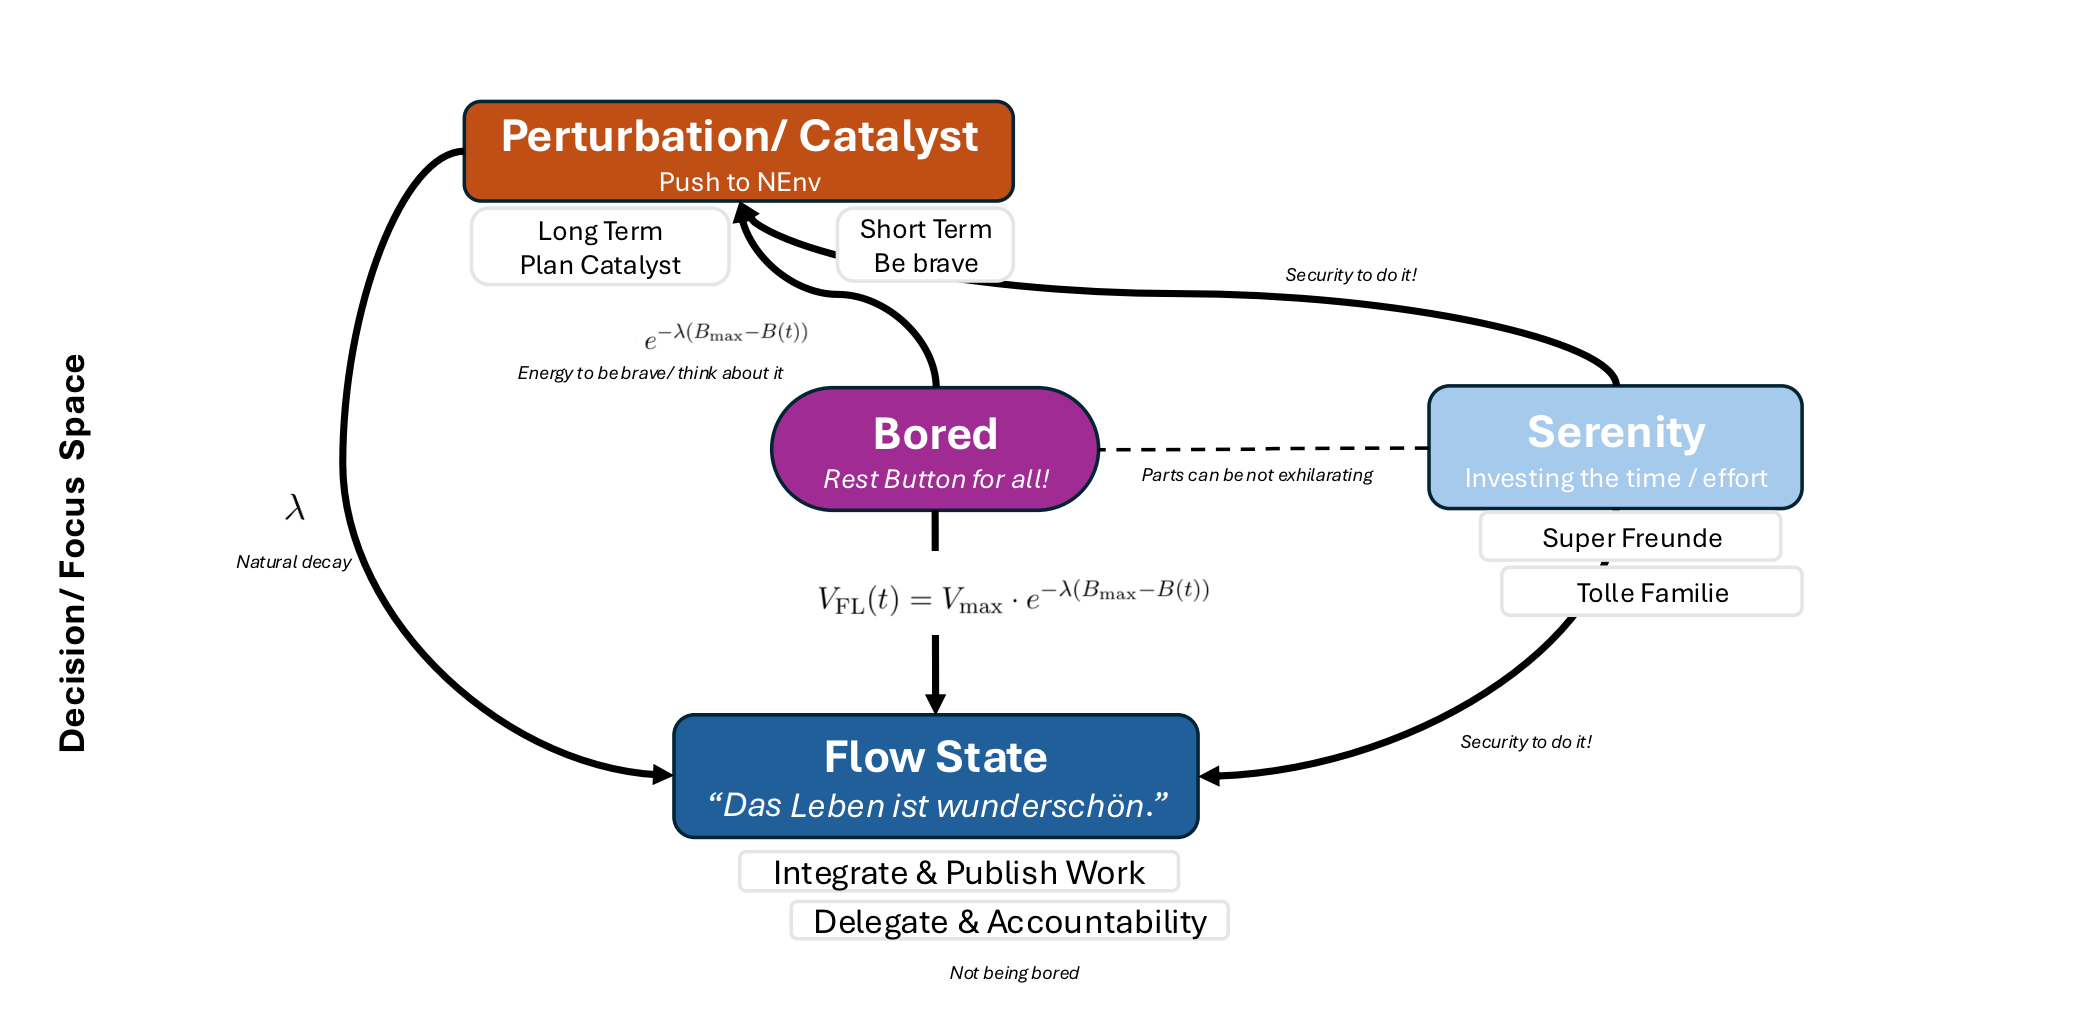
\includegraphics[scale=0.5]{attachment/chapter_OWN/DSci_Rubic__Personal_III}  
	\caption{Decision and Focus Space (Desired and Necessary Feelings)}  
\end{figure}  
